%======================= SRT FOR IMAGE INDEXING ===========================

\renewcommand{\D}{\mathcal{X}} %data domain
\renewcommand{\N}{{D}} %vector size
\renewcommand{\bb}[1]{\boldsymbol {#1}} %\textbf{}
\renewcommand{\muu}{\bb{\mu}}

\graphicspath{{img/str/}}

\chapter{Surrgate Text Representation of Visual Features for Fast Image Retrieval}
\label{ch:str}

%%% ABSTRACT
% The great success of visual features learned from deep neural networks has led to a significant effort to develop efficient and scalable technologies for image retrieval. Nevertheless, its usage in large-scale Web applications of content-based retrieval is still challenged by their high dimensionality.
% To overcome this issue, some image retrieval systems employ the product quantization method to learn a large-scale visual dictionary from a training set of global neural network features. These approaches are implemented in main memory, preventing their usage in big-data applications.
% The contribution of the work is mainly devoted to investigating some approaches to transform neural network features into text forms suitable for being indexed by a standard full-text retrieval engine such as Elasticsearch. The basic idea of our approaches relies on a transformation of neural network features with the twofold aim of promoting the sparsity without the need of unsupervised pre-training.
% We validate our approach on a recent convolutional neural network feature, namely \acrfull{rmac}, which is a state-of-art descriptor for image retrieval. Its effectiveness has been proved through several instance-level retrieval benchmarks.
% An extensive experimental evaluation conducted on the standard benchmarks show the effectiveness and efficiency of the proposed approach and how it compares to state-of-the-art main-memory indexes.

Search engines on the Web have in the past achieved great results in terms of efficiency thanks to the use of inverted index technology.
This development was not as rapid in the case of retrieval of other forms of expression such as images.
This was initially due in part to the ineffectiveness of hand-crafted features used by instance-level and content-based image retrieval.
However, since 2014 we have had a great development of new learned features obtained by training neural networks -- in particular \acrfullpl{cnn}.
In consequence, the remarkable development in the effectiveness of these features has not been matched by a similar development in image retrieval systems; why?
We do not have a clear answer.
One reason could be that people are not very interested in searching for image content on the Web and as a result, major Web search service providers have not invested many resources in this regard.
On the other hand, if the image retrieval were simple and above all scalable as that of the text, perhaps today we would have seen a greater development of these services.

The aim of this article is to explore new approaches to make image retrieval as similar as possible to text so as to reuse the technologies and platforms exploited today for text retrieval without the need for dedicated access methods.
In a nutshell, the idea is to use image representation extracted from a \gls{cnn}, often referred to as \emph{deep features}, and to transform them into text so that they can be indexed with a standard text search engine.

The application focus of this work is on a scenario of image retrieval in a large-scale context, with an eye to scalability.
This aspect is often overlooked by the literature, most of the image retrieval systems are designed to work in main memory and many of these cannot be distributed across a cluster of nodes~\cite{navarro2016new}.
Many techniques present in literature try to tackle this problem by heavily compressing the representation of visual features to adapt more and more data to the secondary memory.
However, these approaches to indexing are not able to scale because sooner or later response times become unacceptable as the size of the data to be managed increases.

Moreover, we must not neglect to consider the effort that it takes to design and implement from scratch an image retrieval system that provides, in addition to the above mentioned requirements, also others such as: allowing simultaneous update and searching, providing support for incremental indexing and for CRUD (Create, Read, Update, and Delete) operations, etc.

In particular, our general approach is based on the transformation of deep features, which are (dense) vectors of real numbers, into sparse vectors of integer numbers.
The transformation in integers is necessary to deal with textual representations of the vectors, as it will be explained better below, in which the components of the vectors are in fact translated by ``term frequency'' of these textual representations.
Sparseness is necessary to achieve sufficient levels of efficiency exactly as it does for search engines for text documents.
To obtain this twofold result, we will analyze two approaches: one based on permutations and one based on \acrfull{sq}.

The present paper is the evolution of previous works~\cite{amato2014mi,gennaro2010approach,amato2016deep,amato2017efficient,amato2018large}.
In~\cite{amato2014mi}, the idea of representing metric objects as permutations of reference objects to construct an inverted index that allows us to perform approximate nearest neighbor queries has been presented.
In~\cite{gennaro2010approach}, this method has been extended by transforming permutations into surrogate text representations and allowing us to take advantage of a standard text search engine without having to implement the inverted index.
\citet{amato2016deep} introduced the idea of deep permutations that applies to the deep feature vectors and in which the components of the vectors themselves are permuted.
\citet{amato2017efficient,amato2018large} presented an extension of the technique of deep permutations, in the former using the surrogate text representation and \gls{rmac}, and in the latter taking into account the negative components of \gls{rmac}.
In~\cite{amato2018large}, we have also proved that this general approach can be implemented on top of Elasticsearch by showing how such a retrieval system is able to scale to multiple nodes.
In the earlier attempt~\cite{amato2016large}, we have presented a preliminary draft of quantization approach on deep features extracted from the Hybrid CNN\footnote{\url{http://github.com/BVLC/caffe/wiki/Model-Zoo}}, which is less effective but has the advantage of being partly sparse.

The original contribution of the present work consists in introducing a new approach of surrogate representation for deep features based on \emph{\gls{sq}}.
We present this approach in a unified framework of representation of deep features using surrogate text together with the technique based on deep permutations, and we compare it with the \gls{sq} technique.
We have also extended the experimental evaluation by adding two more benchmarks and, regarding efficiency, we also considered the size of the indexes as well as their percentage of use.

The rest of the paper is organized as follows: \ref{sec:str:related-work} surveys the relevant related work.
% \ref{sec:str:background} provides a brief background about the Deep Features.
In \ref{sec:str:surrogate}, the main contribution of this paper, namely the Surrogate Text Representation is presented.
\ref{sec:str:experiments} shows experimental results, and finally \ref{sec:str:conclusion} gives concluding remarks.
\ref{tab:str:notation} summarizes the  notation used throughout this manuscript.


\section{Related Work}
\label{sec:str:related-work}
To frame our work in the context of scientific literature, we refer to the survey of \citet{zheng2018sift}, which organizes the literature according to the codebook size, i.e. large/medium-sized/small codebooks.
Although this organization, according to the authors, is relevant to local features (which were defined as ``sift-based'' by the authors), we think it can be extended to deep features.
We think our work belongs to medium-sized (or even large-sized codebooks), which rely on their sparsity to exploit inverted indexes and the trade-off between accuracy and efficiency is a major influencing factor.

In this respect, the scientific literature devoted to mitigating the complexity of computing the matching between local features and based on the generation of visual words, i.e.\ \acrfull{bow}, are very close to our work in the spirit.
If we limit ourselves to consider only the works that exploit the sparsity of the BoW model (originated from a work by \citet{sivic2003video}), \citet{philbin2007object} use an inverted index on secondary memory to implement a scalable visual object-retrieval system based on the SIFT descriptor.
We refer the reader to the survey of \citet{zheng2018sift} for more information about other approaches that quantize local features into visual words.
In the following discussion, we concentrate our attention on techniques that try to deal with deep features with an inverted index.

A permutation-like approach, which relies on the use of special anchor objects called pivots, were used in PPP-Codes index~\cite{novak2015large} to index a collection of 20 million images processed by a deep convolutional neural network.
However, the proposed approach relies on an index specifically developed to manage permutations in secondary memory called \emph{recursive Voronoi partitioning}.

\citet{liu2015indexing} proposed a framework that adapts the BoW model and inverted table to deep feature indexing, which is similar to the one we propose.
However, for large-scale datasets, they have to build a large visual dictionary that employs the product quantization method to learn it from a training set of global deep features.
This approach also uses a specialized index that combines inverted table and hashing codes.
Moreover, it has been tested only with sparse outdated deep features that exhibited low accuracy.

Some other works try to treat the features in a convolutional layer as local features~\cite{arandjelovic2015netvlad,yue2015exploiting}.
This way, a single forward pass of the entire image through the \gls{cnn} is enough to obtain the activation of its local patches, which are then encoded using \acrfull{vlad}.
A similar approach uses the BoW encoding instead of \gls{vlad} to take advantage of sparse representations for fast retrieval in large-scale databases.
However, although authors claim that their approach is very scalable in terms of search time, they did not report any efficiency measurements and experiments have been carried out on datasets of limited size.

\citet{mohedano2016bags} quantized the deep features coming from a \gls{vgg}-16 pre-trained network with a codebook of size 25k and employed an inverted index for efficiency.
Also in this case, although authors claim that their BoW-based representation is highly sparse, allowing for fast retrieval using inverted indices, no experimental evidence was offered.

An approximate nearest neighbor algorithms based on \acrfull{pq}, which exploits an inverted index is presented in~\cite{jegou2011product}.
In \gls{pq}, the original vector is divided into $M$ sub-vectors which are then independently quantized.
A codebook is learned via $k$-means for each of the $M$ sub-division, and each sub-vector is compressed by storing the nearest centroid index.
% In particular, the FAISS library \cite{johnson2017billion} is further improvement of the above approach, which is an implementation of PQ-compressed inverted indexes, denoted IVFPQ.
In particular, we focus on \gls{pq}-compressed inverted indexes, denoted IVFPQ, which are implemented in the open source FAISS library \cite{johnson2017billion}.
In IVFPQ, the feature space is partitioned into $N$ Voronoi cells, each associated with a particular posting list of the inverted file.
Each posting list contains the \gls{pq}-compressed difference between samples belonging to that cell and its centroid.
When building the index, both the cell centroids and the \gls{pq}-compression codebooks have to be pretrained on a subset of the data.
When querying the index, FAISS probes the posting lists of the $P$ Voronoi cells nearest to the query, and it reconstructs the samples using the codebooks.
In the section devoted to the experimental evaluation, we will discuss the performance of FAISS in comparison with our approach.

\begin{table}
\begin{tabularx}{\linewidth}{rX}
\toprule
\textsc{Symbol} & \textsc{Definition} \\
\midrule
$\D$                                           & Data domain \\ \addlinespace[0.5em]
$o,\, o_i \in \D$                              & Data objects \\ \addlinespace[0.5em]
$\v,\, \v_i \in \R^{\N}$                       & $\N$-dimensional data vectors \\ \addlinespace[0.5em]
$\e \in \R^{\N}$                               & Constant vector $[1,\dots, 1]$ \\ \addlinespace[0.5em]
$q \in \D$, $\q \in \R^{\N}$                   & Query  \\ \addlinespace[0.5em]
$d(\cdot, \cdot)$                              & Distance function $d: \D \times \D \to \R+$ \\ \addlinespace[0.5em]
$\ell_2(\cdot, \cdot), \, \|\cdot\|_2$         & Euclidean distance, Euclidean norm  \\ \addlinespace[0.5em]
$S_{\rho}(\cdot, \cdot)$                       & Spearman rho distance \\ \addlinespace[0.5em]
$sim_{cos}(\cdot, \cdot)$                      & Cosine similarity \\ \addlinespace[0.5em]
$\{\tau_1, \dots, \tau_n\}$                    & Codebook \\ \addlinespace[0.5em]
$n \in \mathbb{N}$                             & Codebook size \\ \addlinespace[0.5em]
$f(\cdot)$                                     & Mapping of data objects into integer vectors (term frequencies) \\ \addlinespace[0.5em]
$\text{STR}_f(o),\, t_o$                       & \acrfull{str} of the object $o$ \\ \addlinespace[0.5em]
$\cup$                                         & Space-separated concatenation operator \\ \addlinespace[0.5em]
$\{p_1\ldots p_n\}\subset\D$                   & Set of pivots \\ \addlinespace[0.5em]
$\Pi_{o} \in \mathbb{N}^n$                     & Pivot permutation of $o \in \D$ \\ \addlinespace[0.5em]
$\Pi_{o}^{-1} \in \mathbb{N}^n$                & Inverted permutation of $o \in \D$ \\ \addlinespace[0.5em]
$\tilde{\Pi}_{\v}$                             & \acrfull{dp} of $\v \in \R^{D}$ \\ \addlinespace[0.5em]
$\tilde{\Pi}^{-1}_{\v} \in \mathbb{N}^n$       & Inverted \gls{dp} of $\v\in \R^{D}$ \\ \addlinespace[0.5em]
$k \in \mathbb{N}$                             & Permutation-prefix length \\ \addlinespace[0.5em]
$\tilde{\Pi}^{-1}_{\v,k} \in \mathbb{N}^n$     & Inverted truncated \gls{dp} of $\v\in \R^{D}$ \\ \addlinespace[0.5em]
$R \in \R^{\N \times \N}$, $\muu \in \R^{\N} $ & Random rotation matrix, translation vector \\ \addlinespace[0.5em]
$s \in \R$                                     & \acrlong{sq} factor ($s>1$) \\ \addlinespace[0.5em]
$\gamma \in \mathbb{N}$                        & thresholding parameter \\ \addlinespace[0.5em]
$\v^+ \in \R^{2\N  }$                          & \gls{crelu} of the vector $\v$ \\ \addlinespace[0.5em]
$M \in \mathbb{N}$                             & Number of sub-vectors in which a vector is divided in the \gls{pq} approach \\ \addlinespace[0.5em]
$N \in \mathbb{N}$                             & Number of Voronoi cells used in the \gls{pq} approach \\ \addlinespace[0.5em]
$P \in \mathbb{N}$                             & Number of Voronoi cells used to probe the posting list in the \gls{pq} approach \\ \addlinespace[0.5em]
$C$                                            & Code size (memory occupied by a sample) in the \gls{pq} approach \\ \addlinespace[0.5em]
$S_\text{DB}$                                  & Query selectivity (average fraction of database accessed per query) \\ \addlinespace[0.5em]
$C_\text{DB}$                                  & Query cost (average number of bytes accessed per query) \\ \addlinespace[0.5em]
$B_\text{DB}$                                  & Total size of the database in bytes \\ \addlinespace[0.5em]
$\delta_i, \hat{\delta_i} \in \R$              & Density of $i$-th dimension of a set of data vectors \\ \addlinespace[0.5em]
$ n_i \in \mathbb{N}$                          & Number of elements in the $i$-th posting list \\
\bottomrule
\end{tabularx}
\caption{Notation used throughout this chapter.}
\label{tab:str:notation}
\end{table}

%\section{Background}
%\label{sec:str:background}

%\subsection{Deep Features}
%\label{sec:deepfeatures}
% TODO? check if useful in background chapter
% Recently, a new class of image descriptor, built upon Convolutional Neural Networks, have been used as an effective alternative to descriptors built using local features such as SIFT, ORB, BRIEF, etc.
% CNNs have attracted an enormous interest within the Computer Vision community because of the state-of-the-art results achieved in challenging image classification tasks such as the ImageNet Large Scale Visual Recognition Challenge (\url{http://www.image-net.org}).
% In computer vision, CNNs have been used to perform several tasks, including image classification, as well as image retrieval \cite{donahue2013decaf,babenko2014neural} and object detection \cite{girshick2014rich}, to cite some.
% Moreover, it has been proved that the representations learned by CNNs on specific tasks (typically supervised) can be transferred successfully across tasks \cite{donahue2013decaf,razavian2014cnn}.
% The activation of neurons of specific layers, in particular the last ones, can be used as features to semantically describe the visual content of an image.

%In order to extract Deep Features, we used a trained model publicly available for the popular Caffe framework \cite{jia2014caffe}. Many deep neural network models, in particular trained models, are available for this framework\footnote{\url{https://github.com/BVLC/caffe/wiki/Model-Zoo}} .
%Among them, we chose the HybridNet for several reasons: first, its architecture is the very same of the famous AlexNet \cite{krizhevsky2012imagenet}; second, the HybridNet has been trained not only on the ImageNet subset used for ILSVRC competitions (as many others), but also on the Places Database \cite{zhou2014learning}; last, but not least, experiments conducted on various datasets demonstrate the good transferability of the learning \cite{zhou2014learning,chandrasekhar2015practical,azizpour2015generic}.
%We decided to use the activation of the first fully connected layer, the fc6 layer, given the results reported on \cite{donahue2013decaf,babenko2014neural,chandrasekhar2015practical}.

%The activations at the fc6 layer is a vector of 4,096 of floats. Generally, the rectified linear unit (ReLU) is used to bring to zero all negative activation values. In this way, feature vectors contain only values greater or equal to zero. Feature vectors are sparse so that on average about 75\% of elements are zero.
%\noindent {\large \textbf{R-MAC Features}}\\
%\subsection{R-MAC Features}
%\label{sec:rmacfeatures}
% Recently, image descriptors built upon activations of convolutional layers
% have shown brilliant results in image instance retrieval
% \cite{razavian2014visual, babenko2015aggregating, tolias2015particular}.


%Tolias et al. \cite{tolias2015particular} proposed the R-MAC (Regional Maximum Activations of Convolutions) feature representation, which encodes and aggregates several regions of the image in a dense and compact global image representation.
%To compute an R-MAC feature, an input image is fed to a fully convolutional network pre-trained on ImageNet.
%The output of the last convolutional layer is max-pooled over different spatial regions at different position and scales, obtaining a feature vector for each region.
%These vectors are then $\ell_2$-normalized, PCA-whitened, $\ell_2$-normalized again, and finally aggregated by summing them together and $\ell_2$-normalizing the final result.
%The obtained representation is an effective aggregation of local convolutional features at multiple position and scales that it can be compared with the cosine similarity function.

% \cite{gordo2016end} built on the work of \cite{tolias2015particular}
% and inserted the R-MAC feature extractor in an end-to-end differentiable
% pipeline in order to learn a representation optimized for visual instance
% retrieval through back-propagation.
% The whole pipeline is composed of a fully convolutional neural network,
% a region proposal network, the R-MAC extractor, and PCA-like dimensionality
% reduction layers, and it is trained using a ranking loss based on image triplets.
% The obtained pipeline can extract an optimized R-MAC feature representation
% that outperforms methods based on costly local features and spatial geometry verification.

% An additional performance boost is obtained using state-of-the-art deep
% convolutional architectures, such as very deep residual networks \cite{he2015deep},
% and aggregating descriptors extracted at multiple resolutions. A multi-resolution R-MAC descriptor is obtained feeding the network with images at different resolutions and then aggregating the obtained representations by summing them together and then performing a final $l2$-normalization.


%%LUCIA: ma questa parte non sarebbe meglio metterla negli esperimenti? qun mi sembra stoni un po'..
% In our work, we used the ResNet-101 trained model provided by Gordo et al. \cite{gordo2016end} as an R-MAC feature extractor, which has been shown to achieve the best performance on standard benchmarks.
% We extracted the R-MAC features using fixed regions at two different scales as proposed in \cite{tolias2015particular} instead of using the region proposal network.
%Defined $S$ as the size in pixel of the minimum side of an image, we computed the multi-resolution descriptor aggregating the ones extracted at $S=550$, $800$ and $1,050$, resulting in a dense $2048$-dimensional real-valued image descriptor.

%%%%%%%%%%%%%%%%%%

%Lucia%
\section{Surrogate Text Representation} % (?? o un titolo migliore)
\label{sec:str:surrogate}
As we explained in the introduction, we aim to index and search a data set of feature vectors by exploiting off-the-shelf text search engines.
So our main goal is to define a family of transformations that map a feature vector into a textual representation without the need for tedious training procedures.
Of course, we also require that such transformations preserve as much as possible the proximity relations between the data, i.e.\ similar feature vectors are mapped to similar textual documents.

This basic idea was firstly exploited in~\cite{gennaro2010approach}, where the authors defined the \acrfull{str} to represent a generic metric object, i.e.\ an object living in a space where a distance function is defined~\cite{zezula2006similarity}.
The \gls{str} of an object is a space-separated concatenation of some alphanumeric codeword selected from a pre-defined dictionary.
The original approach uses a permutation-based indexing technique (further described in \ref{subsec:str:deep-permutations}) to generate the textual encoding.
Here, we observe that a surrogate text representation for an object $o$ of a data domain $\D$ can be obtained more generally by defining a transformation
\begin{align}
	f : \D &\to \mathbb{N}^n\\
	o &\mapsto \bb{f}_o=[f_o^{(1)}, \dots, f_o^{(n)}] \,,
\end{align}
where $\bb{f}_o$ will act as the vector of the \glspl{tf} of a synthetic text document $t_o$ with respect to a dictionary of $n$ words.
Specifically, given a dictionary $\{\tau_1, \dots, \tau_n\}$ and the transformation $f$, we define the surrogate text $ t_o=\text{STR}_f(o)$ as
\begin{equation}
	\text{STR}_f(o)=\bigcup_{i=1}^n\,\bigcup_{j=1}^{f_o^{(i)}} \tau_i
\end{equation}
where, by abuse of notation, we denote the space-separated concatenation of the codewords with the union operator $\cup$.
Thus, by construction, the integer values of the $i$-th component of the vector $\bb{f}_o$ is the frequency of the codeword $\tau_i$ in the text $\text{STR}_f(o)$.
For example, given $\bb{f}_o=[1,3,0,2]$ and a codebook $\{\tau_1=``A'',\,  \tau_2=``B'',\, \tau_3=``C'', \,\tau_4=``D''\}$, we have $\text{STR}_f(o)=``A \, B \, B \, B \, D \, D''$.

The rational of this approach is that a full-text search engine based on the \emph{vector space model} \cite{salton1986introduction} will generate a vector representation of the $\text{STR}_f(o)$ by counting the number of occurrences of the words in it, i.e.\ the term frequencies.
In facts, these systems transform the text into vector representations using the well-known \gls{tf} scheme and practically use the dot product as a function of similarity between vectors.
So, the abstract transformation $f(\cdot)$ represents a function that exactly generates the vectors that are internally represented by the search engine in the case of the simple term-weighting scheme.
Using this representation, the search engine indexes the text by using inverted files, i.e.\ each object $o$ is stored in the posting lists associated to the codewords appearing in $\text{STR}_f(o)$ (\ref{fig:str:posting-list}).

\begin{figure}
\centering
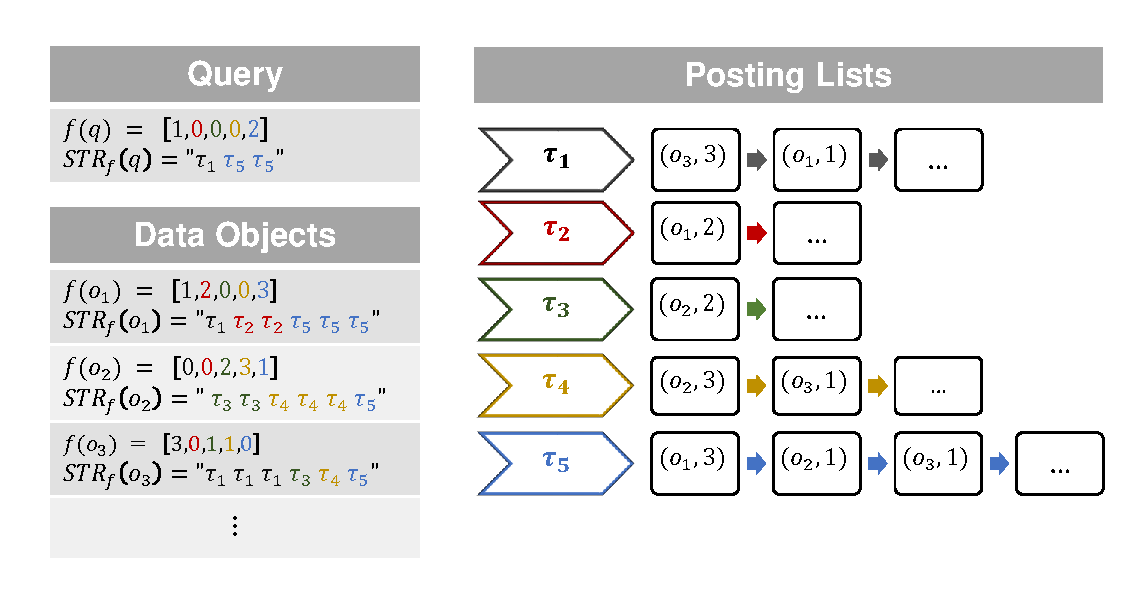
\includegraphics[trim=0mm 5mm 0mm 0mm,clip, width=1\textwidth]{PostingList.pdf}
\caption{Example of the \gls{str} encodings for a query object $q$ and three data objects $o_1, o_2, o_3$.
The \glspl{str} are indexed using posting lists.
The posting lists accessed at query time are the only ones associated to the codewords comparing in the surrogate text representation of the query.
For example, given the query $\text{STR}_f(q)=$''$\tau_1\, \tau_5\, \tau_5$'', the posting lists accessed are just those related to the codewords $\tau_1$ and $\tau_5$.}
\label{fig:str:posting-list}
\end{figure}

Ideally, the transformation $f(\cdot)$ should be
\begin{enumerate}
	\item \emph{order-preserving}:  the ranked results to the query $q$ (obtained by searching the original space $\D$) exactly correspond to the ranked results to the text query $\text{STR}_f(q)$ (obtained by searching the surrogate text space);%
\footnote{Note that to compare a query with a set of objects we can use either a \emph{distance} or a \emph{similarity} function.
In the former case, we search for the objects with the greatest similarity to the query.
In the latter case, we search for the objects with the lowest distance from the query. A similarity function is said to be \emph{equivalent} to a distance function if the ranked list of the results to a query is the same.}
	\item \emph{sparsifying}: for any $o \in\D$, the vector $f(o)$ is sparse.
\end{enumerate}

The order-preserving property guaranties we do not loose any solutions when using the textual representation with respect to the results that would be obtained using the original data representation.
However, having this property is quite impossible in practice since it is likely that any hand-crafted function $f(\cdot)$ introduces some approximations when transforming the data objects into term-frequency vectors.
Thus, the \emph{effectiveness} of a \gls{str}-based retrieval system highly depends on how good the transformation $f(\cdot)$ is in preserving the object similarities.
The sparsifying property, instead, is requested for \emph{efficiency} issues since each data object $o$ will be stored in as many posting lists as the number of the non-zero elements in $f(o)$.
Having dense vectors means that the search based on the inverted index would be significantly more expensive than the sequential scan, moreover also the index size would be much bigger than the original dataset.
The ideal case is having uniformly sparse vectors so that the length of each posting list is approximately the same.

Unfortunately, the sparsifying property is in contrast with the order-preserving one since the former naturally introduces some approximations in the vectors, which basically translates our problem into a trade-off between effectiveness (score approximation) and efficiency (posting-list length).

In this paper, we are interested in indexing and searching \emph{$\N$-dimensional vectors} originally compared with the dot product, such as the \gls{rmac} descriptors. Note that, in this case, $\D=\R^{\N}$ and the order-preserving property with respect to dot product can be expressed as
\begin{equation}
\forall\, \q,\v_1,\v_2 \in \R^{\N} \quad	\bb{q}\cdot \bb{v_1} \leq \bb{q}\cdot \bb{ v_2} \Rightarrow f(\bb{q})\cdot f(\bb{v_1}) \leq f(\bb{q})\cdot f(\bb{v_2}).
\end{equation}

Below we present two text transformation techniques that can be used in this context: a Permutation-Based approach and Scalar Quantization approach.
We then discuss how to achieve sparse representations for these two approaches.

\subsection{Permutation-Based Approach}
\label{subsec:str:deep-permutations}

The basic idea of permutation-based indexing techniques is to represent feature objects as permutations of a set of identifiers.
Traditionally, the permutation representations are built using the identifiers of a set of reference objects as permutants.
This approach is more general than the one we adopt in this article, as it admits as objects not only vectors but more generally metric objects for which there exists a distance function providing a measure of the closeness of two data objects.

Formally, given a domain $\D$, a distance $d:\D\times \D\to \R+$, and a fixed set  $\{p_1\ldots p_n\}\subset\D$ of \emph{reference objects} (or \emph{pivots}), we define a permutation-based representation $\Pi_{o}$ (briefly \emph{permutation}) of an object $o\in \mathcal{D}$ as the sequence of pivots identifiers sorted in ascending order by their distance from $o$ \cite{mtap12,amato2014some}.
In other words, the permutation-based representation $\Pi_{o}=$ $[\Pi_{o}(1), \ldots , \Pi_{o}(n)]$ lists the pivot identifiers $\{1, 2, \ldots, n\}$ in an order such that $\forall\, i,j \in \{1,\ldots, n\}$
\begin{equation}
\begin{matrix}
& & d(o,p_{\Pi_{o}(i)}) <    d(o,p_{\Pi_{o}(j)})\, \\
\Pi_{o}(i)< \Pi_{o}(j)\qquad &\Leftrightarrow\qquad & or \\
& &\left(\, d(o,p_{\Pi_{o}(i)}) =    d(o,p_{\Pi_{o}(j)})\, \wedge\, (i<j)\, \right) \,,
\end{matrix}
\end{equation}
where $p_{\Pi_o(j)}$ indicates the pivot at position $j$ in the permutation associated with object $o$.
An equivalent permutation-based representation is the \emph{inverted permutation}, defined as  $\Pi^{-1}_{o}=[\Pi_{o}^{-1}(1), \Pi_{o}^{-1}(2),\dots , \Pi_{o}^{-1}(n)]$, where $\Pi_{o}^{-1}(i)$ denotes the position of a pivot $p_i$ in the permutation $\Pi_{o}$, so that $\Pi_o(\Pi_o^{-1}(i))=i$.
Thus, the coordinate $i$ in the permutation $\Pi_{o}$ is the identifier of the pivot at $i$-th position in the ranked list of the nearest pivots to $o$;
the value at the coordinate $i$ in the inverted representation $\Pi^{-1}_{o}$ is the rank of the pivot $p_i$ in the list of the nearest pivots to $o$.

%The inverted permutation $\Pi^{-1}_{o}$ is a vector that we also refer to as \emph{vector of permutations}.
The inverted representation of the permutations is often used in practice since it allows us to easily define most of the distance functions usually used to compare permutations, such as the Spearman rho and the Spearman Footrule distances.
%Permutations are generally compared using Spearman rho, Kendall Tau, or Spearman Footrule distances.
In this work, we use the Spearman rho, which can be defined as the Euclidean distances between inverted permutations: $S_\rho (\Pi_{o_1},\Pi_{o_2})=\ell_2(\Pi^{-1}_{o_1},\Pi^{-1}_{o_2})$.

The original \gls{str} approach, \cite{gennaro2010approach} is based on a double transformation process.
First, each data object $o$ is transformed in a permutation vector (the inverted permutation) $\Pi^{-1}_{o}$ using the approach presented above, and then it transforms the permutation into a textual representation $t_o$.
The textual representation is obtained by associating each pivot $p_i$ with an unique alphanumeric codeword $\tau_i$ and the permutation $\Pi^{-1}_{o}$ with a sequence of codewords.
Specifically, the text $t_o$ is built in such a way that the occurrence of the codeword $\tau_i$ in it reflects the closeness of the pivot $p_i$ to the object $o$: the lower the value $\Pi^{-1}_{o}(i)$ the higher the frequency of the term $\tau_i$ in the document $t_o$.
Formally, the original \gls{str} approach uses the transformation
$
f_{perm} : o \mapsto n\e - \Pi^{-1}_{o} %\bb{f}_o=[f_o^{(1)}, \dots, f_o^{(n)}]
$,
%\begin{align}
%f_{perm} : \D &\to \mathbb{N}^n\\
%o &\mapsto n\e - \Pi^{-1}_{o} %\bb{f}_o=[f_o^{(1)}, \dots, f_o^{(n)}]
%\end{align}
where $\e=[1,\dots, 1]$ is the constant vector.
Therefore,
\begin{equation}
\text{STR}_{f_{perms}}(o)=\bigcup_{i=1}^n\,\bigcup_{j=1}^{n-\Pi^{-1}_{o}(i)} \tau_i.
\end{equation}

The rational behind this approach is that if two objects are very close one to the other, they will sort the set of pivots in a very similar way, and thus the corresponding permutations/text representations will be close as well.
Note that we have no theoretical guarantees that the transformation
\begin{align}
\Pi^{-1} : (\D,d) &\to (\mathbb{N}^n, \ell_2)\\
o &\mapsto \Pi^{-1}_{o}
\end{align}
is order-preserving in a strict sense, however several works \cite{amato2014mi,gonzalez2008effective,esuli2009mipai} experimentally proved that the rankings obtained in the permutation space are good approximations of the rankings obtained in the original space.
Moreover, it can be easily proved that the cosine similarity between any two term frequency vectors is a monotonic transformation of the squared Euclidean distance between the associated inverted permutations: $sim_{cos}(f_{perms}(o_1), f_{perms}(o_2))=\alpha - \beta\,\ell_2(\Pi^{-1}_{o_1},\Pi^{-1}_{o_2})^2 $, where $\alpha \in R{}$, $\beta \in \R+$ are constants (see \cite{vadicamo2016using,vadicamo2018enhancing}).
Therefore, a ranking obtained using the cosine similarity on term frequency vectors is equivalent to that obtained in the permutation space using the Spearman rho distance, which in turn is an approximation of the ranking obtained in the original data space.

So far, we have presented the general approach of \gls{str} based on the traditional permutation representations.
However, when objects to be indexed are \emph{real-valued vectors}, as in the case of deep features, we can exploit the deep permutations technique~\cite{amato2016deep} that allows to generate the permutations at very low computational cost by avoiding the calculations of the distances between the pivots and the objects to be represented.
Moreover, \citet{amato2016deep} shown that this encoding is more effective than the traditional permutation-based representation for both multimedia retrieval and similarity search tasks.
In the deep permutations approach, the permutants are the indexes of the elements of the deep feature vectors rather that a predefined set of pivots.
Specifically, the deep permutation of a feature vector $\v \in \R^{n}$ is obtained by sorting the \emph{indexes} of the elements of $\v$, in descending order with respect to the corresponding element values. In other words, the \emph{\gls{dp}} $
\tilde{\Pi}_{\v} = [ \tilde{\Pi}_{\v}(1), \ldots, \tilde{\Pi}_{\v}(n) ]
$
of a deep feature $\v$ is the permutation of the indexes $\{1,\dots, n\}$ such that
\begin{equation}
\forall i=1, \cdots, n-1, \quad \v\( \tilde{\Pi}_{\v}(i) \) \geq \v \( \tilde{\Pi}_{\v}(i+1) \) \,,
\end{equation}
where we use the notation $\v(j)$ to indicates the $j$-th element of $\v$.
So the index $i$ appears before index $j$ in the permutation $\tilde{\Pi}_{\v}$ if the value $\v(i)$ is greater than or equal to $\v(j)$.
Equivalently, using the inverted representation $
\tilde{\Pi}^{-1}_{\v} = [ \tilde{\Pi}^{-1}_{\v}(1), \ldots, \tilde{\Pi}^{-1}_{\v}(n) ]
$, we have that $\tilde{\Pi}^{-1}_{\v}(i) \leq \tilde{\Pi}^{-1}_{\v}(j)$ if $\v(i)\geq \v(j)$.
Using the approach introduced above, similarly to the traditional \gls{str} technique, we can define the transformation
$
f_\text{DP} : \v \mapsto n\e -\tilde{\Pi}^{-1}_{\v}
$ to associate a term frequency vector to each data object.

Suppose, for instance, that the feature vector is $\v = [0.1, 0.3, 0.4, 0, 0.2]$ (in reality, the number $n$ of dimensions may be thousands).
The deep permutation encoding of $\v$ is $\tilde{\Pi}_{\v}=[3, 2, 5, 1, 4]$, that is permutant (index) 3 is in position 1, permutant 2 is in position 2, permutant 5  is in position 3, etc.
In facts, $\v(3) = 0.4$ is the biggest value in $\v$, $\v(2) = 0.3$  is the second biggest element value, and so on.  The corresponding inverted deep permutation is $\tilde{\Pi}^{-1}_{\v} = [4, 2, 1, 5, 3]$, that is permutant (index) 1 is in position 4, permutant 2 is in position 2,  permutant 3 is in position 1, etc.
The term frequencies vector will be $f_\text{DP}(\v) = [1, 3, 4, 0, 2]$, and thus $\text{STR}_{f_\text{DP}}(\v)=``A\, B\, B\, B \, C \, C\, C\, C\, E\, E"$.

\subsection{Scalar Quantization-Based Approach}
\label{subsec:str:sq}
In this section, we propose an alternative approach to provide a surrogate text representation for feature vectors.
The idea behind our \acrfull{sq} approach is to map the real-valued vector components independently into a smaller set of integer values which act as the term frequencies of a predefined set of codewords.
%This is very similar to the way Scalar Quantization works (?????). %questa frase c'era già ma non ho capito cosa volevi dire
However, as for more generic \gls{pq}, the \gls{sq} has mainly the purpose of making a compact representation suitable for approximate nearest neighbor search.

The first step in our approach is the application of an order-preserving transformation to the vectors, that basically is a random rotation of the feature vectors.
This step is important for efficiency issues since it prevent to have unbalanced posting lists in the inverted file.
%Without this step, the posting list of the inverted index would be unbalanced which would therefore affect its performance.
To understand why, remember that in our approach each component of the vectors is associated with a posting list in which each post stores the \emph{id} of the vector and the value of the component itself, if nonzero.
Therefore, if on average some component is nonzero for many data vectors then the corresponding posting list will be accessed many times, provided that the queries follow the same distribution of the data.
The ideal case occurs when the component share exactly the same distribution (same mean and variance is sufficient).
To this end, we apply a roto-translation transform to the entire set of data vectors.
In this way, we try to increase to cases where the dimensional components of the features vectors have same mean and variance, with mean equal to zero.
This last constraint is because we want then sparsify the vectors, but this aspect is further investigated in the next subsection.

An important aspect of the roto-translation transform is that it preserves the ranking when we search using the kNN approach by ordering the vectors on the basis of their Euclidean distance to the query.
Moreover, if applying the roto-translation to all the data objects and just the rotation to the query we have an ordering preserving transformation with respect to the dot-product: given a rotation matrix $R \in \R^{\N \times \N}$ and a vector $\muu \in \R^{\N}$, then
\begin{equation}
\forall\, \q, \v_1, \v_2 \in \R^{\N} \quad	\q \cdot \v_1 \leq \q \cdot \v_2 \Rightarrow R\q\cdot R(\v_1 - \muu) \leq R\q\cdot R(\v_2 - \muu) \,.
\end{equation}
%Every transformation that does not violate the previous inequality can be applied to $f_q$ and $fv_i$ without changing the relative rankings of vectors with respect to the query.
We found that a good transformation is the random rotation:
\begin{align}
\v &\to R(\v - \muu) \\
\q &\to R \q \,,
\end{align}
where $R$ is a \emph{random} orthogonal matrix ($\|R\|_2 = 1$) and $\muu \in \R^{\N}$ can be arbitrary chosen.
The random rotation helps to distribute information equally over the vector components.

The next step is transforming the rotated vectors into term frequency vectors.
We do it by quantizing the vectors so that posting entries will contain numeric values proportional to the float values of the deep feature entries.
Specifically, we use the transformation $\w \to \lfloor s\w \rfloor$ where $\lfloor \rfloor$ denotes the floor function and $s$ is a multiplication factor $> 1$ that works as a \emph{quantization factor}.
This process introduces a quantization error due to the representation of float components in integers.
However, as we will see, this error does not affect the retrieval effectiveness.

In summary, the \gls{sq}-based \gls{str} is obtained using the transformation
$
f_\text{SQ} : \v \mapsto \lfloor s R(\v -\muu)\rfloor
$.

For instance, suppose after the random rotation we have the feature vector $\v = [0.1, 0.3, 0.4, 0, 0.2]$, by adopting a multiplication factor $s = 10$, we obtain the term frequencies vector will be $f_\text{SQ}(\v) = [1, 3, 4, 0, 2]$, and thus $\text{STR}_{f_\text{SQ}}(\v)=``A\, B\, B\, B \, C \, C\, C\, C\, E\, E"$.

\subsection{Sparsification}
The two approaches presented above are intended to encode a vector of real numbers into a vector of integers preserving as much as possible the order with respect to the the dot product.
However, this approach does not solve the problem that in most cases these vectors are dense, which means having low efficiency performance if the inverted files are used to index the textual documents.
%This is because the next step will be to encode these integer vectors into textual documents to index with standard text-based techniques (based on inverted indices).
In order to sparsify the term frequency vectors, that is to cancel the less significant components of the vectors, we must accept a further loss in precision.
To achieve this we propose two ways: keep the top-$k$ larger components of the vector or maintain components above a certain threshold $1/\gamma$ by zeroing all the others.
Where $\gamma \in \mathbb{N}$ is the parameter we use to control the sparseness of the thresholded feature.
The first approach (\emph{top-$k$}) is better suited to the permutation-based approach and the latter (\emph{thresholding}) to the \gls{sq} approach.

The top-$k$ approach on the permutation-based encoding can be seen as the selection of a fixed-length prefix of the permutations.
This approach works well since it is assumed that the greatest information is in the first $k$ elements of the permutation, i.e.\ the identifiers of the closest pivots to the object to be represented.
It is equivalent to say that instead of using the full-length inverted permutation $\tilde{\Pi}^{-1}_{\v}$  we use the \emph{truncated inverted permutation}
\begin{equation}
\tilde{\Pi}^{-1}_{\v,k}(i) = \begin{cases}
                                \tilde{\Pi}^{-1}_{\v} (i) & \text{if} \quad \tilde{\Pi}^{-1}_{\v}(i) \leq k \\
                                k+1                       & \text{otherwise}
                             \end{cases} \,.
\end{equation}
Note that, in the permutation-based indexing context, using the positions of the {nearest} $k$ out of $n$ pivots often leads to obtaining better or similar effectiveness then using the full-length permutation \cite{amato2014mi,amato2014some}, resulting also in a more compact data encoding.
To transform the truncated inverted permutation into a term frequency vectors, we use $f_{\text{DP},\,k} : \v \mapsto (k+1)\e -\tilde{\Pi}^{-1}_{\v,k}$.

The thresholding adopted for \gls{sq} simply discards by setting to zero the dimension of the vector $\v$ having absolute values above a specified threshold:
\begin{equation}
\v_{\gamma} (i) = \begin{cases}
                    \v (i) & \text{if} \quad \v (i) \geq \frac{1}{\gamma} \\
                    0      & \text{otherwise}
                  \end{cases} \,,
\end{equation}
where $\v(i)$ indicates the i-th dimension of the feature vector $\v$.
This approach is optimal when we have many components near or equal to zero;
hus, we exploit the roto-traslation transform seen above to center the mean values of each dimension to zero.


%Claudio%
% \section{Text Transformations}
% As we explained in the introduction, our goal is to define a family of transformations of the feature vectors that allow us to generate codes, without the need for tedious training procedures, suitable for text indexing that have as main characteristic that of being as sparse as possible. The proposed approach relies on the use of search engine based on the vector space model. These systems transform the text into vector representations using the well-known TF scheme and practically use the dot product as a function of similarity between vectors. Since as a precondition we require that the function of similarity between the vectors of the original features is also the dot product, another important aspect of these vector transformation is that we want as much as possible as order-preserving with respect to dot product. This property is unfortunately in contrast with the sparsity one, which basically translates into a trade-off between effectiveness (score approximation) and efficiency (posting-list length).
% The order-preserving property can be formally defined as follow.
% Given a query and two vectors $f_q, fv_1, fv_2 \in \mathbb{R}^{N}$, we say that the transformation $\tau(fv_i) \in \mathbb{R}^{N}$ is order-preserving with respect to dot product if:

% \begin{equation}
% f_q \cdot fv_1 > f_q \cdot fv_2 \rightarrow \tau(f_q) \cdot \tau(fv_1) > \tau(f_q) \cdot \tau(fv_2)
% \end{equation}\label{eq:orderpres}

% It is important to understand that the abstract transformation function $\tau()$ represents a function that exactly generates the vectors that are internally represented by the search engine based on the vector model.

% Below we present two text transformation techniques: a Permutation-Based approach and Scalar Quantization approach.

 %\subsection{Permutation-Based Approach}\label{subsec:str:deep-permutations}
% The basic idea of permutation-based indexing techniques is to represent feature objects as permutations built using a set of reference object identifiers as permutants.
% This approach is more general than the one we adopt in this article, as it admits as objects not only vectors but more generally metric objects for which the only requirement is to have a distance function of $d$, as defined here below.
% Given a domain $\mathcal{D}$,
% a \emph{distance function} $d:\mathcal{D}\times\mathcal{D}\rightarrow\mathbb{R}$,
% and a fixed set of reference objects $P=\{p_1\ldots p_n\}\subset\mathcal{D}$ that we call \emph{pivots},
% we define a permutation-based representation $\Pi_{o}$ (briefly \emph{permutation}) of an object $o\in \mathcal{D}$ as the sequence of pivots identifiers sorted in ascending order by their distance from $o$ \cite{mtap12}.

% \sloppy Formally, the permutation-based representation
% %$\Pi_{o}=(\Pi_{o}(1), \Pi_{o}(2), ... , \Pi_{o}(n))$
% $\Pi_{o}=$ $(\Pi_{o}(1), \ldots , \Pi_{o}(n))$
% lists the pivot identifiers in an order such that
% %$\forall j \in \{1, 2, \ldots, n-1\}, \;d(o,p_{\Pi_{o}(j)}) \leq
% $\forall j \in \{1,  \ldots, n-1\}, \;d(o,p_{\Pi_{o}(j)}) \leq
% d(o,p_{\Pi_{o}(j+1)})$,
% where $p_{\Pi_o(j)}$ indicates the pivot at position $j$ in the permutation associated with object $o$.
% If we denote as $\Pi_{o}^{-1}(i)$ the position of a pivot $p_i$, in the
% permutation of an object $o\in \mathcal{D}$,
% so that $\Pi_o(\Pi_o^{-1}(i))=i$, we obtain the equivalent \emph{inverted} representation of permutations %$\Pi^{-1}_{o}$:
% $\Pi^{-1}_{o}=(\Pi_{o}^{-1}(1), \ldots, \Pi_{o}^{-1}(n)).$
% %$$\Pi^{-1}_{o}=(\Pi_{o}^{-1}(1), \Pi_{o}^{-1}(2), ... , \Pi_{o}^{-1}(n))$$
% In $\Pi_{o}$ the value in each position of the sequence is the identifier of the pivot in that position. In the inverted representation $\Pi^{-1}_{o}$, each position corresponds to a pivot and the value in each position corresponds to the rank of the corresponding pivot.
% The inverted representation of permutations $\Pi^{-1}_{o}$, is a vector that we refer to as \emph{vector of permutations}, and which allows us to easily define most of the distance functions between permutations.
% Permutations are generally compared using Spearman rho, Kendall Tau, or Spearman Footrule distances.

% So far, we have presented the general approach of permutation-based indexing. However, when objects to be indexed are \emph{real-valued vectors} as in the case of deep features, we can use the approach presented in \cite{amato2016deep}. It allows us to generate a sequence of identifiers not associated with pivots. The basic idea is as follows. Permutants are the indexes of elements of the deep feature vectors. Given a deep feature vector, the corresponding permutation is obtained by sorting the indexes of the elements of the vector, in descending order with respect to the values of the corresponding elements. Suppose for instance the feature vector is $fv=[0.1,0.3,0.4,0,0.2]$ (in reality, the number of dimensions is 2,048 or more). The permutation-based representation of $fv$ is $\Pi_{fv}=(3,2,5,1,4)$, that is permutant (index) 3 is in position 1, permutant 2 is in position 2, etc. The vector of permutations introduced above is therefore $\Pi^{-1}_{fv}=(4,2,1,5,3)$, that is permutant (index) 1 is in position 4, permutant 2 is in position 2, etc.

%  \subsection{Scalar Quantization-Based Approach}\label{subsec:str:sq} \noindent
% The idea behind Scalar Quantization is to map the real-valued vector components independently into a smaller set of output values  which make up as codebook. This is very similar to the way Scalar Quantization works. However, as for more generic Product Quantization, the Scalar Quantization has mainly the purpose of making a compact representation suitable for approximate nearest neighbor search.

% The first step in our approach is the application of order-preserving transformations to the vectors. Without this step, the posting list of the inverted index would be unbalanced which would therefore affect its performance. To understand why, remember that in our approach each component of the vectors is associated with a posting list in which each post stores the \emph{id} of the vector and the value of the component itself if nonzero. Therefore if some component in average is nonzero for many vector it will be accessed many times, provided that the queries follow the same distribution. The ideal case occurs when the component share exactly the same distribution (same mean and variance is sufficient). To this end, we apply the same roto-translation transform to the entire set of vectors. In this way, we try to increase to cases where the mean of the components have same mean and variance, with mean equal to zero. This last constraint is because we want then sparsify the vectors, but this aspect is studied in the next subsection.

% An important aspect of this transformation, as stressed above, is that we have to preserve the ranking when we search using the kNN approach by ordering the vectors on the basis of their dot products. Every transformation that does not violate the previous inequality can be applied to $f_q$ and $fv_i$ without changing the relative rankings of vectors with respect to the query. We found that a good transformation is the random rotation:

% $$ \bar{fv_i} = Rfv_i $$

% where $R \in \mathbb{R}^{N \times N}$ is an random orthogonal matrix ($|R| = 1$) and $\mu \in \mathbb{R}^{N}$ can be arbitrary chosen. Note that also the query must be rotated.

 %\subsection{Thresholding}

% The two approaches presented above are intended to encode a vector of real numbers into a vector of integers preserving as much as possible the order with respect to the the dot product. This is because the next step will be to encode these integer vectors into textual documents to index with standard text-based techniques (based on inverted indices). However, this approach does not solve the problem that in most cases these vectors are dense, which means having low efficiency performance with the inverted files.
% In order to sparsify the vectors, that is to cancel the less significant components of the vectors, we must accept a further loss in precision. To achieve this we can proceed in two ways: keep the first $k$ components larger than the vector (top-$k$) or maintain components (thresholding) above a certain threshold $Q$ by zeroing all the others. The first approach is better suited to the permutation-based approach and the latter to the \gls{sq} approach.

% top-$k$ approach can be seen as application of a fixed-length prefix of the permutations, which has the aim of reducing the size of the permutation representations. This approach works well since it is assumed that the greatest information is in the first $k$ elements of the permutation. The thresholding adopted for \gls{sq} is optimal when we have many components near or equal to zero, and, to maximize this effect, we try to use the roto-traslation transform seen above.

% \subsection{Surrogate Text Representation}\label{sec:srt}

% So far, we have only seen theoretical approaches to vector encoding and we only vaguely mentioned, at the beginning of this section, something about how to transform these encodings into text. The basic idea is to exploit the approach presented in \cite{gennaro2010approach}, called surrogate text representation (SRT), in which the integer value represented by the component of the vector is encoded in the frequency of a codeword that is associated with the component itself. The rational is that a full-text search engine will generate a vector representation of \gls{str} counting the number of occurrences of words in SRT, i.e., their term-frequencies. Moreover, the similarity of full-text search engine is usually based on dot product, which is exactly what we wanted to use. This approach of SRT generation is straightforward for the case of Thresholding method, in case of deep permutation a more fuhrer step is needed,  which consists in complementing the rank vector of permutations, with the number of permutants plus one. For instance, if our rank vector is $\Pi^{-1}_{fv}=(4,2,1,5,3)$., its complemented version is $\overline{P}i^{-1}_{fv}=(6-4,6-2,6-1,6-5,6-3)=(2,4,5,1,3)$.

%%%%%%%%%%%%%%%%%%%%%%%%%%%%%%%%%%%%%%%%%%

\subsection{Dealing with Negative Values}

In order to index \gls{rmac} features and represent them in the vector space model of text retrieval, we encode each dimension of the \gls{rmac} features as a different codeword, and we use the \gls{tf} field to represent a single value of our feature vector.
However, the \gls{tf} must be positive (no search engine admits negative TFs even if this in principle would be possible), nonetheless, both negative and positive elements contribute to informativeness.
In the two approaches presented above, this produces two different negative effect, but fortunately the solution we adopt is the same for both.
In the \gls{sq} case, negative quantized components are not admitted for construction; in the deep permutation-based approach, negative components are neglected since they always fall behind the positive ones in the ordering.
In order to prevent this imbalance towards positive activations at the expense of negative ones, we use the \gls{crelu} transformation~\cite{shang2016understanding}.
It simply makes an identical copy of vector elements, negate it, concatenate both original vector and its negation, and then apply \gls{relu} altogether.
More precisely the \gls{crelu} of the vector $\v$ is defined as $\v^+ = \text{ReLU}([\v, -\v])$, where the $\text{ReLU}(\cdot) = max(\cdot, 0)$ is applied element-wise.
After applying \gls{crelu}, we applied either $f_\text{DP}$ or $f_\text{SQ}$ (or their sparsifying versions) to $\v^+$ as described in the previous sections.
%More precisely, we denote ReLU as $[\cdot]^+ = max(\cdot, 0)$, and define \gls{crelu} of the vector $\v$ as $\v^+ = ([\v]^+,[-\v]^+)$.%everything proceeds in the case of vectors with positive components with the two seen approaches.

For instance, if $\v = [0.1, -0.3, -0.4, 0, 0.2]$, the \gls{crelu} applied on $\v$ is $\v^+ = [0.1, 0, 0, 0, 0.2, 0, 0.3, 0.4, 0, 0]$.
If using the deep permutations approach, the corresponding inverted permutation is $\Pi^{-1}_{\v^+} = [4, 5, 6, 7, 3, 8, 2, 1, 9, 10]$ (ties take random positions) and thus $f_\text{DP}(\v^+) = [6, 5, 4, 3, 7, 2, 8, 9, 1, 0]$.
For completeness, we report the example also for the case of a spasifying factor $k=4$, for which we have $\Pi^{-1}_{\v^+,4} = [4, 5, 5, 5, 3, 5, 2, 1, 5, 5]$ and $f_{\text{DP},\, k}(\v^+) = [1, 0, 0, 0, 2, 0, 3, 4, 0, 0]$.
%For completeness we report the example for the case of  deep permutations approach the inverted permutation is  .
If we apply the \gls{sq} technique to the same vector $\v^+$, with the values of $\gamma = 5$ and $s=10$, we obtain $f_{\text{DP}, \, k}(\v^+) = [0, 0, 0, 0, 2, 0, 3, 4, 0, 0]$. % TODO check: should be f_SQ?

Notice that in general, the \gls{crelu} operation is lossy since the dot product between vectors is not preserved, i.e.\ $\v_1 \cdot \v_2 \leq \v_1^+ \cdot \v_2^+$.
However, this transformation allows us to apply the deep permutation approach without completely neglecting the negative activations of the \gls{rmac} features.
%After applying the \gls{crelu} to the vectors $fv$, the rest of the procedure is the same as the deep permutation on vectors $fv+$, and everything else proceeds as for the conventional deep permutation approach.

\section{Experimental Evaluation}
\label{sec:str:experiments}

The aim of this section is to assess the performance of the proposed solution in a content-based retrieval task both in terms of effectiveness and efficiency.
To this end, we are able to evaluate the approximation introduced with respect to the exact similarity search algorithm against the impact of this approximation with respect to the user perception of the retrieval task.
%\subsection{Experimental Settings}
% \todo{Questo copia-incolla va cambaito}
%For assessing the proposed technique in a pure similarity search task, we used the CNN Features extracted as discussed in \ref{sec:deepfeatures} from the \emph{Yahoo Flickr Creative Commons 100 Million dataset (YFCC100M)} \cite{thomee2016yfcc100m}.
%The assessment of the proposed algorithm of a multimedia information retrieval task was performed using
We extracted the \gls{rmac} features from the images of two different benchmarks: \emph{INRIA Holidays} and \emph{Oxford Buildings}.
% TODO riferire background
% INRIA Holidays \cite{jegou08} is a standard benchmark for image retrieval consisting in a collection of 1,491 images representing a large variety of scene type (natural, man-made, water, etc). The authors of INRIA Holidays selected 500 queries and manually identified a list of qualified results for each of them. In the literature, this benchmark is extended with the distractor dataset MIRFlickr including 1M images called MIRFlickr1M (\url{http://press.liacs.nl/mirflickr/}).
% Oxford Buildings \cite{Philbin07} is composed of 5,062 images of 11 Oxford landmarks downloaded from Flickr. A manually labeled groundtruth is available for five queries for each landmark, for a total of 55 queries. As for \emph{INRIA Holidays}, we merged the dataset with the distraction dataset Flickr100k including 100k images \footnote{\url{http://www.robots.ox.ac.uk/~vgg/data/oxbuildings/}}.

We compared the performance of our approach with state-of-the-art approximate nearest neighbor algorithms based on \gls{pq} FAISS \cite{johnson2017billion}, which we presented in \ref{sec:str:related-work}.
In the implementation of FAISS, the number of Voronoi cells $N$ controls the number and length of the postings lists, while the number of \gls{pq} sub-quantizer $M$ controls the amount of memory occupied by a sample, also known as code size $C$.
Moreover, we directly choose the code size $C$, and $M$ is set accordingly by the software.
Since FAISS is an in-memory index, $C$ is usually set to the maximum code size to fit the whole dataset we want to index in main memory.
While $N$ and $C$ are fixed parameter chosen at indexing time, the number of nearest neighbor Voronoi cells to probe $P$ can be adjusted at query time and can be tuned to control the effectiveness-efficiency trade-off.

For a fair comparison, we used a configuration for FAISS which gives the best trade-off between effectiveness and efficiency for each dataset, choosing a relatively big code size ($C=1,024$ for Holidays, $C=512$ for Oxford) and optimal number of Voronoi cells ($N = 16$k for Holidays and $N=1.5$k for Oxford).
However, these configurations have long index training times and a large memory footprint (for 1M images and $C=1,024$, FAISS requires about 1GB in main memory, against about 0.7GB of our solution in secondary memory in the larger configuration for $k=400$), and this could limit its scalability, especially in systems with limited main memory.

We generated different sets of permutations from the original features using different values of $k$ for the permutation-based approach (i.e., we consider top-$k$ truncated permutations) and $\gamma$ for the \gls{sq} approach.
For each configuration, we measured the \acrfull{map} obtained and the query execution times for each configuration.
As the goal of our approach is to work in a context of large scale image search, in the experiments, we report the \gls{map} (on the $y$-axis) in function of either the \emph{Query Selectivity} $S_\text{DB}$, i.e.\ the average fraction of database accessed per query, or the \emph{Query Cost} $C_\text{DB}$, i.e. average number of bytes accessed per query.
If the total size of the database in bytes is $B_\text{DB}$, then the following equality holds: $C_\text{DB} = B_\text{DB} \cdot S_\text{DB}$.


% Previous work \cite{icmr17} compares mAP values in function of the sparsity of the vectors to be indexed.
% We believe that the level of sparsity introduced by the truncation at $K$ may be misleading in measuring the number of accesses to the inverted file.
% In fact, \gls{crelu} increases the dimensionality and the sparsity of a vector, but only the original elements of the vector are actually stored in our index.
% Hence, the sparsity could be artificially increased without changing the number of elements really accessed at query time.
The query selectivity for \gls{str} techniques can easily be derived as follows.
Given a database comprised of $N$ $D$-dimensional objects ($D=2,048$ for $\v$ in the case of \gls{rmac}), the query selectivity $S_\text{DB}$ is defined as the fraction of the $N \cdot D$ elements accessed to answer a query.
Let $\delta_i$ the density of $i$-th dimension computed as the fraction of samples in the database having a non-zero $i$-th dimension.
Given a query $\q$, we access the $i$-th posting list only if the $i$-th dimension of $ \q$ is non-zero, which is true with probability $\delta_i$ since query and dataset objects share the same distribution.
The number $n_i$ of elements contained in the $i$-th posting list equals the number of elements of the database having non-zero $i$-th dimension, that is $n_i = \delta_i \cdot N$.
Hence, the number of elements accessed to answer a query is
\begin{equation}
\sum_{i=1}^D \delta_i \cdot n_i \,,
\end{equation}
because $i$-th posting list contains $n_i$ elements, and we access it with $\delta_i$ probability.
Thus, we can compute the query selectivity
\begin{equation}
S_\text{DB} = \frac{1}{ND} \sum_{i=1}^D \delta_i \cdot n_i = \frac{1}{D} \sum_{i=1}^D {\delta_i}^2\,.
\end{equation}
Similarly, in the case of the \gls{crelu}-ed vector $\v^+$, the number of dimensions (and thus posting lists) doubles, but the number of total non-zero elements stored in the index is still at most $N \cdot D$.
Thus,
\begin{equation}
S_\text{DB} = \frac{1}{D} \sum_{i=1}^{2D} \hat{\delta_i}^2 \,,
\end{equation}
where $\hat{\delta}_i$ denotes the density of the $i$-th dimension of the \gls{crelu}-ed version of the dataset.

Note that, in a surrogate text representation, we associate a distinct codeword to each dimension of the vector, and the smaller the query selectivity is, the more balanced are the posting lists of the inverted index.
The greater is $k$, the lower is the sparsity, and hence the greater is the \emph{\gls{map}} and the query selectivity.
Since we are dealing with an approximate approach, the brute-force \gls{map}, i.e.\ the one computed with the original features and a sequential scan of the entire database, can be considered as an upper-bound.

\begin{figure}

\begin{subfigure}{\linewidth}
\centering
\caption{\centering mAP vs Query Selectivity for the Holidays + MIRFlickr1M dataset.}%
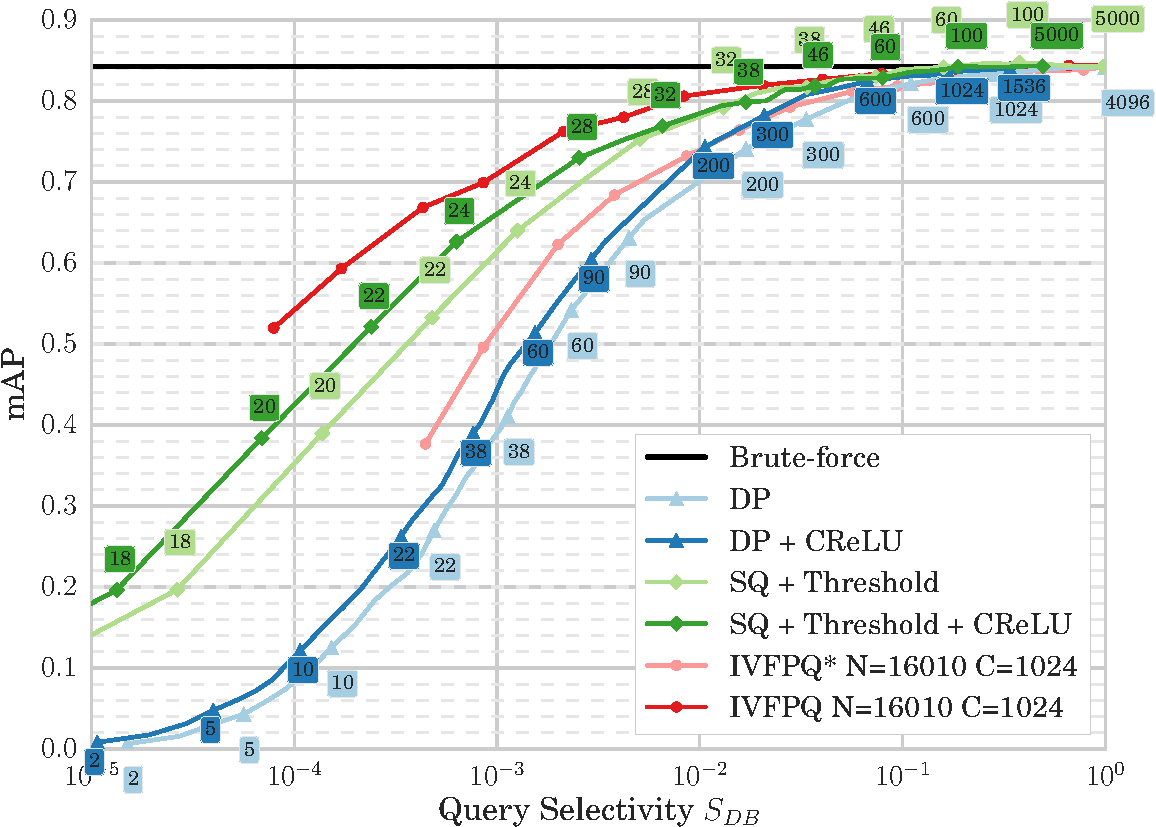
\includegraphics[width=\linewidth,height=0.44\textheight,keepaspectratio]{plot_Holidays_MIRFlickr1M_QSelectivity}
\end{subfigure}\\[4ex]
\begin{subfigure}{\linewidth}
\centering
\caption{\centering mAP vs Query Cost for the Holidays + MIRFlickr1M dataset.}%
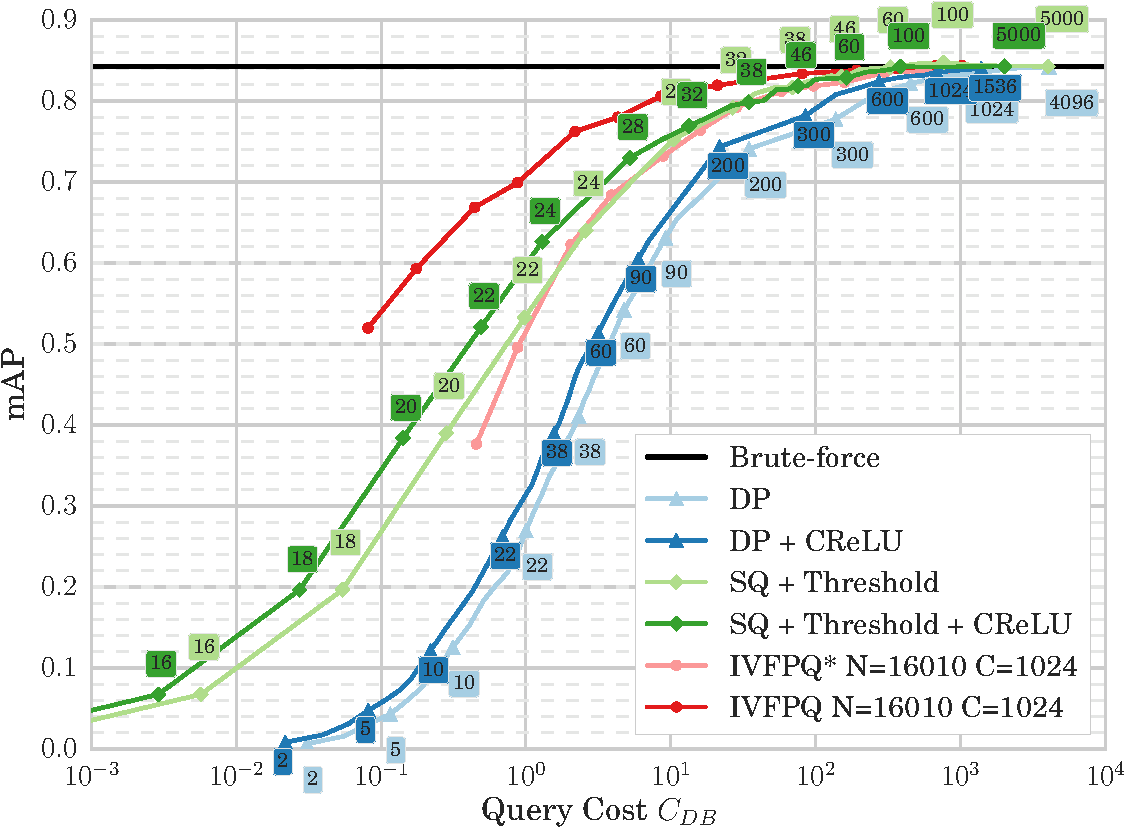
\includegraphics[width=\linewidth,height=0.44\textheight,keepaspectratio]{plot_Holidays_MIRFlickr1M_QCost}
\end{subfigure}
\end{figure}%
%
\begin{figure}
\ContinuedFloat
\begin{subfigure}{\linewidth}
\centering
\caption{\centering mAP vs Query Selectivity for the Oxford + Flickr100k dataset.}%
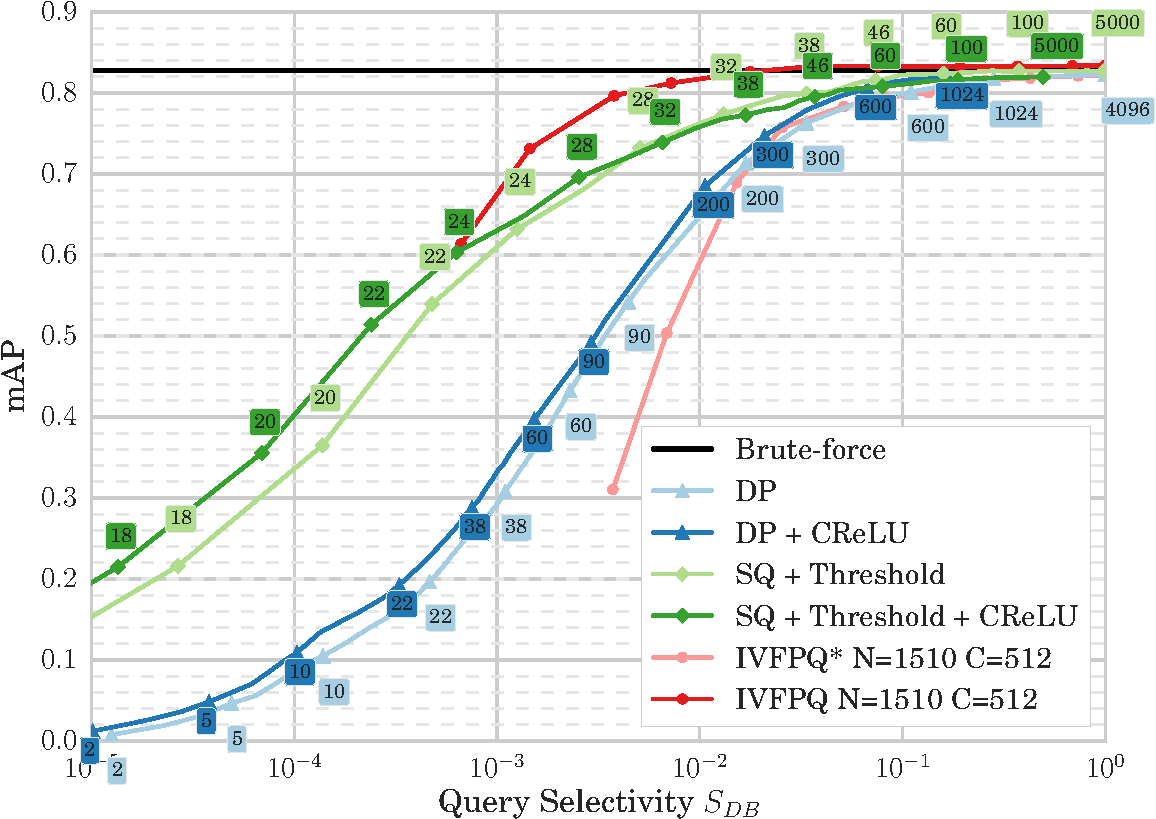
\includegraphics[width=\linewidth,height=0.39\textheight,keepaspectratio]{plot_Oxford_Flickr100k_QSelectivity}
\end{subfigure}\\[4ex]
\begin{subfigure}{\linewidth}
\centering
\caption{\centering mAP vs Query Cost for the Oxford + Flickr100k dataset.}%
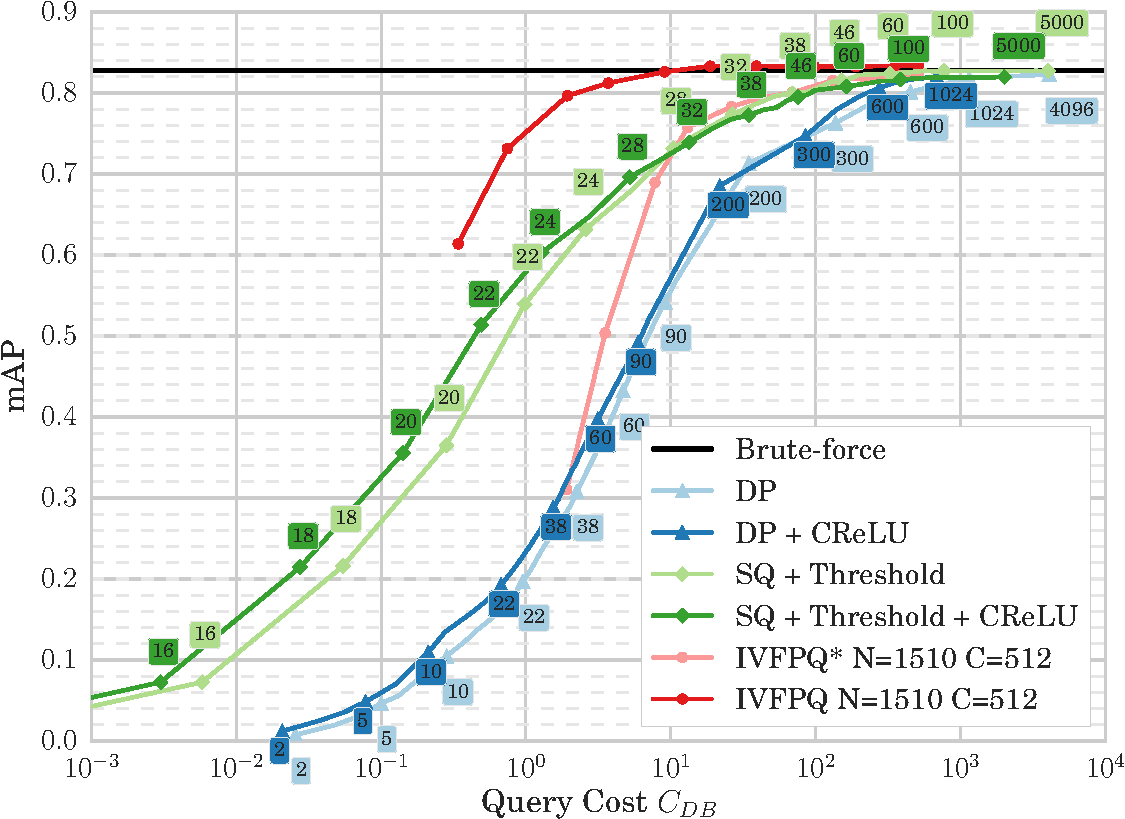
\includegraphics[width=\linewidth,height=0.39\textheight,keepaspectratio]{plot_Oxford_Flickr100k_QCost}
\end{subfigure}

\caption{Comparison of the performance of our method and \gls{pq}-compressed inverted-file-based indexes (FAISS) on Holidays + MIRFlickr1M (a-b) and on Oxford + Flickr100k (c-d), in terms of mAP and query selectivity/cost trade-off.
The curves are obtained varying $k$ (for deep permutations), $\gamma$ (for thresholded \gls{sq}), and the number of Voronoi cell accessed $P$ (for IVFPQ).
Values of $k$ and $\gamma$ are reported near each point.
The horizontal line represents the \gls{mAP} obtained using the original \gls{rmac} vectors and performing a sequential scan of all the dataset (brute-force approach).
%For our method, the sparsity of the dataset is given by $\frac{K}{2048}$.
}
\label{fig:str:results}
\end{figure}

\ref{fig:str:results} reports the performance of the evaluated approaches on both datasets.
We can see that we reach satisfactory levels of effectiveness for a query selectivity of $10^{-2}$.
Moreover, we have shown the remarkable advantage of the \gls{crelu} preprocessing on \gls{rmac} vectors in comparison with the deep permutation method applied directly on the original vectors.

We would like to stress two points concerning the experiments on \gls{sq}.
%First, we used a large value of $s$, tending to MAX\_INT, because we noticed that for values of s larger than 100 the effect on performance is really small.
First, we used a large value of $s$ in order to exploit the full range of numbers that can be expressed in term-frequencies integers depending on the search engine implementation employed (we considered a 32-bit integer in our experiments on Elasticseach).
We could analyze the impact on performance for low values of $s$, but we believe that this study is of little relevance because the \gls{str} approach involves using a standard search engine, so we would not have any control over how the integers within the posting lists are effectively implemented by the search engine.
Second, the reported experiments with \gls{sq} without the \gls{crelu} transformation (`SQ + Threshold' line in \ref{fig:str:results}) are simulated, since the components of the vectors can also be negative and thus not implementable with the \gls{str} approach on a standard textual search engine.

We also report the performance of FAISS indexes when varying the number of Voronoi cells probed $P$.
We report two curves related to FAISS which correspond to two different datasets used for learning the codebooks: the indexed dataset itself, on which the mAP evaluation is performed, and an uncorrelated dataset of images.
For the latter, we employed the \gls{t4sa} dataset~\cite{vadicamo2017cross}, a large collection of images collected from the live stream of random 5\% of global tweets using the Twitter Streaming API .
The reason for this choice is to show how the performance of FAISS is sensitive to the specific dataset distribution on which it has been trained.
Indeed, we see the impact of this aspect is really strong, and it could, in real applications, influence the scalability of the system or require continuous codebook adjustments, forcing to re-indexing the data periodically.
Our solution has an intermediate performance but does not require any training procedure and therefore any re-adjustments.

To sum up, based on the results of the experiments we can conclude that the proposed approach, i.e.\ the \gls{sq}, outperforms the deep permutations one.
Note how the \gls{crelu} technique has a negligible impact on the \gls{sq} for suitable values of \gls{map} --- i.e.\ greater than $0.7$.
Therefore, we suggest to use the optimal value for $\gamma=32$, which exhibits good performance both in terms of effectiveness and efficiency.

%%%%%%%%%%%%%%%%%%%%%%%%%%%%%%%%%%%%%%%%%%

\section{Conclusions and Future Works}
\label{sec:str:conclusion}
In this chapter, we proposed a simple and effective methodology to index and retrieve convolutional features without the need for a time-consuming codebook learning step.
To get an idea, consider that FAISS takes about three hours for learning the codebook from about a million \gls{rmac} features with the configuration used in the experiments.
This aspect is often left out by the authors; nevertheless, in the context of Web-scale applications --- in which we frame our work --- we think that not only processing time is a relevant aspect, but also being as independent as possible from data distribution during the indexing phase is a crucial point to be robust to data distribution drifting through time.

Another important aspect of our work is that our technique is completely independent from the technology used for indexing.
We can rely on the latest text search engine technologies, without having to worry about issues related to implementation problems, such as software maintenance, updates to new hardware technologies, bugs, etc.
Furthermore, with our approach, it is possible to include in the image records, in addition to the visual features (which are in textual form), other information such as text metadata, geotags, etc.

We plan to extend our work by investigating the possibility of modifying the \gls{rmac} extraction network to directly learn a ``discretized vector'' similar to the one we get with the proposed hand-crafted method while trying to maximize sparsity and increase the cardinality of the codebook as much as possible.
